%%%%%%%% ICML 2021 EXAMPLE LATEX SUBMISSION FILE %%%%%%%%%%%%%%%%%

\documentclass{article}

% Recommended, but optional, packages for figures and better typesetting:
\usepackage{microtype}
\usepackage{graphicx}
\usepackage{subfigure}
\usepackage{booktabs} % for professional tables
\usepackage{amsmath,amsfonts,amssymb,mathtools}
% hyperref makes hyperlinks in the resulting PDF.
% If your build breaks (sometimes temporarily if a hyperlink spans a page)
% please comment out the following usepackage line and replace
% \usepackage{icml2021} with \usepackage[nohyperref]{icml2021} above.
\usepackage{hyperref}
\allowdisplaybreaks
% Attempt to make hyperref and algorithmic work together better:
\newcommand{\theHalgorithm}{\arabic{algorithm}}

% Use the following line for the initial blind version submitted for review:
\usepackage{icml2022}


\newcommand{\etal}{\textit{et al}.}
\newcommand{\ie}{\textit{i}.\textit{e}., }
\newcommand{\eg}{\textit{e}.\textit{g}. }
\newcommand{\algoname}{\text{Master-User}}
\newcommand{\archi}{\text{Col-NN}}

% If accepted, instead use the following line for the camera-ready submission:
%\usepackage[accepted]{icml2021}

% The \icmltitle you define below is probably too long as a header.
% Therefore, a short form for the running title is supplied here:
\icmltitlerunning{Two Constraints for Online Scalable Recurrent Learning}

\begin{document}

\twocolumn[
\icmltitle{Two Constraints to Scale Unbiased Recurrent Learning}

% It is OKAY to include author information, even for blind
% submissions: the style file will automatically remove it for you
% unless you've provided the [accepted] option to the icml2021
% package.

% List of affiliations: The first argument should be a (short)
% identifier you will use later to specify author affiliations
% Academic affiliations should list Department, University, City, Region, Country
% Industry affiliations should list Company, City, Region, Country

% You can specify symbols, otherwise they are numbered in order.
% Ideally, you should not use this facility. Affiliations will be numbered
% in order of appearance and this is the preferred way.
\icmlsetsymbol{equal}{*}

\begin{icmlauthorlist}
\icmlauthor{Khurram Javed}{to}
\icmlauthor{Haseeb Shah}{to}
\icmlauthor{Rich Sutton}{to,dmorg}
\icmlauthor{Martha White}{to}

\end{icmlauthorlist}



\icmlaffiliation{to}{RLAI Lab, University of Alberta, Edmonton}
\icmlaffiliation{dmorg}{DeepMind, Edmonton}

\icmlcorrespondingauthor{Khurram Javed}{kjaved@ualberta.ca}

% You may provide any keywords that you
% find helpful for describing your paper; these are used to populate
% the "keywords" metadata in the PDF but will not be shown in the document
\icmlkeywords{Machine Learning, ICML}

\vskip 0.3in
]

% this must go after the closing bracket ] following \twocolumn[ ...

% This command actually creates the footnote in the first column
% listing the affiliations and the copyright notice.
% The command takes one argument, which is text to display at the start of the footnote.
% The \icmlEqualContribution command is standard text for equal contribution.
% Remove it (just {}) if you do not need this facility.

%\printAffiliationsAndNotice{}  % leave blank if no need to mention equal contribution
% \printAffiliationsAndNotice{\icmlEqualContribution} % otherwise use the standard text.

\begin{abstract}
% Learning in neural networks requires structural credit-assignment --- identifying parameters that influence a prediction made by the network. For recurrent learning, a parameter can influence a prediction made many steps in the future making credit-assignment challenging. Two popular gradient-based algorithms for structural credit-assignment are (1) Back-propagation Through Time (BPTT) and (2) Real-time Recurrent Learning (RTRL). BPTT requires memory proportional to the length of the input sequence and scales poorly.
% % Additionally, it does not spread the operations for gradient computation uniformly across time. 
% RTRL, on the other hand, can compute gradients in real-time for arbitrarily long sequences using constant memory but is computationally intractable for large networks. In this work, we propose a network architecture --- Columnar Neural Networks (\archi{}) --- and a credit-assignment algorithm --- \algoname --- that allow us to approximate gradients in real-time using $O(n)$ operations and memory per-step. Our method builds on the idea that for modular recurrent networks composed of columns with scalar states it is sufficient for a parameter to track its influence on the state of its own column. As long as connections across columns are sparse, our approximation is close to the true gradient. \archi{} trained with \algoname can be applied for learning recurrent states and for meta-learning using two traces per-parameter.

Online scalable recurrent learning is challenging. Two popular gradient-based methods for recurrent learning are BPTT, and RTRL. BPTT requires processing the complete sequence before computing gradients, and is unsuitable for online updates. RTRL can do online updates, but scales poorly with the number of parameters. In this paper, we propose two constraints that make RTRL scalable. We show that by either decomposing the network into independent modules, or learning a recurrent network incrementally, we can make RTRL scale linearly with the number of parameters. Both compromises result in algorithms with different properties, that can be combined. We show the strengths and weaknesses of the proposed algorithms on a supervised and a prediction learning benchmark.
\end{abstract}

\section{Introduction}
Structural credit-assignment --- identifying how to change network parameters to improve predictions --- is an essential component of learning in neural networks. Effective structural credit-assignment requires tracking the influence of parameters on future predictions. A parameter can influence a prediction in the future in two primary ways. First, for recurrent networks (RNNs), a parameter can influence the internal state of the network which, in turn, can affect a prediction made many steps in the future. Second, if the network is learning online, a parameter can influence the learning updates. These learning updates, in turn, influence predictions made in the future. Structural credit-assignment through recurrent states is called recurrent state learning, whereas through the learning updates is called meta-learning (Schmidhuber,~1987; Bengio~\etal,~1990; and Sutton,~1992). 

Back-Propagation Through Time (BPTT)~(Werbos, 1988; Robinson and Fallside, 1987) is a popular algorithm for gradient-based structural credit-assignment in RNNs. BPTT extends the back-propagation algorithm for feed-forward networks --- independently proposed by Werbos~(1974) and Rumelhart~\etal~(1986) --- to RNNs by storing network activations from prior steps, and repeatedly applying the chain-rule starting from the output of the network and ending at the activations at the beginning of the sequence. BPTT is unsuitable for online learning as it requires memory proportional to the length of the sequence. Moreover, it delays gradient computation until the end of the sequence. For online learning, this sequence can be never-ending or arbitrarily long. 





% The dependence of BPTT on storing activations from past hinders its application to online learning. Additionally, the computation in BPTT is not spread uniformly across time --- the learner accumulates activations for a sequence in the memory and delays the computation of the gradients until the end. This is incompatible with the goal of real-time learning --- the ability to incorporate feedback from the environment quickly for correcting mistakes. 


RTRL --- an alternative to BPTT --- was proposed by Williams and Zipser~(1989). RTRL relies on forward-mode differentiation --- using chain-rule to compute gradients in the direction of time --- to compute gradients recursively. Unlike BPTT, RTRL does not delay gradient-computation until the final step. The memory requirement of RTRL also does not depend on the sequence length. As a result, it is a better candidate for real-time online learning. Unfortunately, RTRL requires maintaining the Jacobian $\frac{\partial h(t)}{\partial \theta}$ at every step, which requires $O(|h||\theta|)$ memory, where $|h|$ is the size of state of the network and $|\theta|$ is the number of total parameters. The Jacobian is recursively updated by applying chain rule as:  
$$\frac{\partial h(t+1)}{\partial \theta} =\frac{\partial h(t+1)}{\partial \theta(t+1)} +  \frac{\partial h(t+1)}{\partial h(t)}\frac{\partial h(t)}{\partial \theta}, $$ 
which requires  $O(|h|^2|\theta|)$ operations and scales poorly to large networks.

% For a more thorough explanation of the memory and time complexity of recurrent state-learning and meta-learning methods using RTRL, see Appendix A. 
 
 

A promising direction to scale gradient-based credit-assignment to large networks is to approximate the gradient. Elman~(1990) proposed to ignore the influence of parameters on future predictions completely for training RNNs. This resulted in a scalable but biased algorithm. Williams and Peng~(1990) proposed a more general algorithm called Truncated BPTT (T-BPTT). T-BPTT tracks the influence of all parameters on predictions made up to $k$ steps in the future. T-BPTT is implemented by limiting the BPTT computation to last $k$ activations and works well for a range of problems~(Mikolov~\etal, 2009, 2010; Sutskever, 2013 and Kapturowski~\etal, 2018). Its main limitation is that the resultant gradient is blind to long-range dependencies. Mujika~\etal~(2018) showed that on a simple copy task, T-BPTT failed to learn dependencies beyond the truncation window. Tallec~\etal~(2017) demonstrated T-BPTT can even diverge when a parameter has a negative long-term effect on a target and a positive short-term effect. 

\begin{figure*}
	\centering
	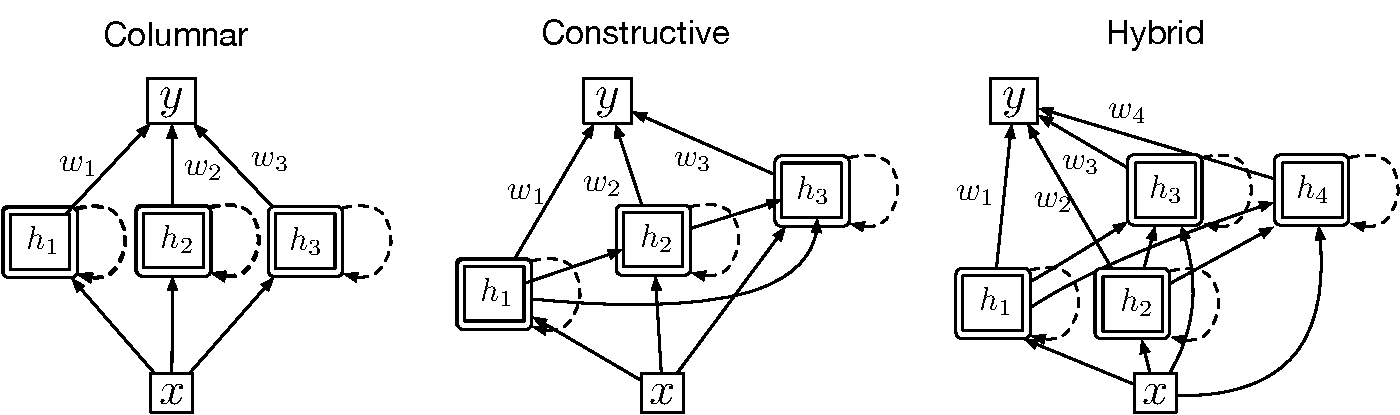
\includegraphics[width=0.8\textwidth]{figures/three_types}
	\caption{TODO: Make the caption concise. Three structures of recurrent neural networks that can be trained without truncation. Recurent networks with a columnar structure can be trained end-to-end using gradients without any truncation, only requiring $O(n)$ operations and memory per step. However, columnar networks do not have hierarchical recurrent features---recurrent features made out of other recurrent features. Constructive networks have hierarchical recurrent features, however must be trained incrementally to prevent bias. Incremental learning is achieved by initializing all $w_i$ to zero, and learning $h_1$, $h_2$, and $h_3$ in order. Finally, columnar and constructive networks can be combined to get a hybrid network. The pairs $(h_1, h_2)$ and $(h_3, h_4)$ do not depend on each other, and can learn in parallel. Hoever, $(h_3, h_4)$ must be learned after $(h_1, h_2)$ have been learned and fixed.}
\end{figure*}

RTRL can also be approximated to reduce its computational overhead. Ollivier~\etal~(2015) and Tallec~\etal~(2017) proposed NoBacktrack and UORO. Both of these algorithms provide stochastic unbiased estimates of the gradient and scale well. However, their estimates have high variance and require extremely small step sizes for effective learning. Cooijmans and Martens~(2019) and Menick~\etal~(2021) showed that, for practical problems, UORO does not perform well due to its high variance compared to other biased approximations. Menick~\etal~(2021) proposed an approximation to RTRL called SnAp-$k$. SnAp-$k$ tracks the influence of a parameter on a state only if the parameter can influence the state within $k$ steps. It first identifies parameters whose influence on a state is zero for $k$ steps and then assumes the future influence to be zero as well. For the remaining parameters, it tracks their influence on all future predictions. The bias introduced by SnAp-k is fundamentally different than the bias introduced by T-BPTT. SnAp-1 can be computationally efficient but introduces significant bias. SnAp-$k$ for $k>1$ reduces bias but can be as expensive as RTRL for dense RNNs.  Menick~\etal~(2021) further proposed using sparse connections as a way to make SnAp more scalable. Connection sparsity reduces the number of parameters that can influence a state within $k$ steps
%  SnAp, combined with sparsity, is a promising research direction.

 Menick~\etal~(2021) showed that for highly sparse networks, SnAp-$k$ reduces the computational requirement of RTRL by over 95\% while keeping bias in check. One limitation of their work is that they do not provide a scalable method to identify parameters that would not influence a state within $k$ steps. Instead, they run the RNN for $k$ steps and look at the full Jacobian $\frac{\partial h(t)}{\partial \theta}$ to determine these parameters. For large networks, computing this Jacobian even once is not possible. Moreover, because they induce sparsity randomly in their networks, the resultant sparsity in the Jacobian is not structured and is not amenable to efficiency gains using existing hardware. Finally, SnAp does not scale well when used in conjunction with deep feature extractors. If internal states operate on a shared representation computed with a deep network with parameters $\theta$, even SnAp-1 could require $O(|\theta||h|)$ memory and $O(|\theta||h|^2)$ operations per-step. Our goal is to design an algorithm that requires $O(|\theta|)$ memory and operations.






% \section{Connections to Neuroscience}

\section{Conclusion and Discussion} 

 

\nocite{sutton1992adapting}
\nocite{finn2017model}
\nocite{kingma2014adam}
\nocite{rumelhart1986learning}
\nocite{werbos1974beyond}
\nocite{werbos1988generalization}
\nocite{li2017meta}
\nocite{javed2019meta}
\nocite{bengio2019meta}
\nocite{williams1989learning}
\nocite{robinson1987utility}
\nocite{vivek}
\nocite{hochreiter1997long}
\nocite{menick2020practical}
\nocite{tallec2017unbiased}
\nocite{cooijmans2019variance}
\nocite{sutskever2013training}
\nocite{elman1990finding}
\nocite{mikolov2009neural}
\nocite{mikolov2010recurrent}
\nocite{ollivier2015training}
\nocite{bengio1990learning}
\nocite{cho2014learning}
\nocite{glorot2010understanding}
\nocite{mujika2018approximating}
\nocite{williams1990efficient}
\nocite{kapturowski2018recurrent}
\nocite{pllr}
\nocite{schmidhuber1987evolutionary}. 
\nocite{glorot2011deep}
\nocite{Tange2011a}
\bibliography{citations}

\bibliographystyle{icml2022}


\onecolumn 
\appendix

%%%%%%%%%%%%%%%%%%%%%%%%%%%%%

\end{document}

